\maketitle
\setcounter{page}{1}
\newpage
\pagenumbering{arabic}
\section{Theorie}
\subsection{Sagnac-Interferometer}
\label{sec:lol}
In Abbildung \ref{fig:1} befindet sich der Aubau desn Sagnac-Interferometers.
\begin{figure}
  \centering
  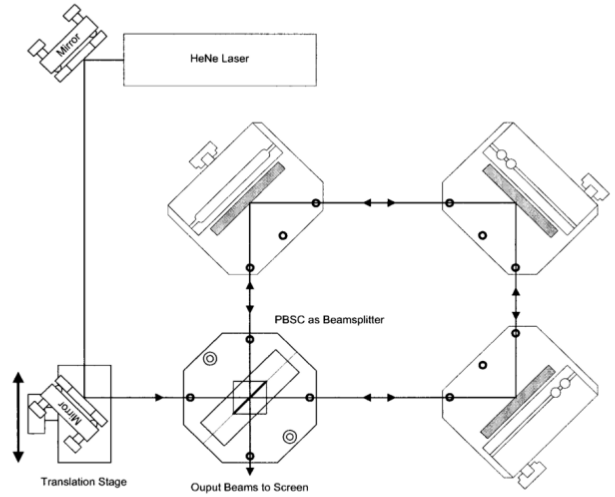
\includegraphics[scale=0.5]{aufbau.png}
  \caption{Schematischer Aufbau des Sagnac-Interferometers. \cite{anleitung}}
  \label{fig:1}
\end{figure}
Zu sehen ist ein Helium-Neon-Laser, dessen Strahl über zwei Steuerspiegel in
ein Rechteckt aus weiteren Spiegeln geleitet wird. Zwischen Steuerspiegeln und
Rechteck befindet sich ein Polarizing Beam-Splitter-Cube (PBSC), welcher aus zwei
rechtwinkligen Prismen, welche an der Hypotenuse zusammengeklebt sind. Dieser PBSC
hat die Eigenschaft, ohne Intensitätsverlust einen unpolarisierten Strahl in
zwei Strahlen mit 90° Winkelunterschied und zueinander senkrechter Polarisation
aufzuspalten. Somit legen die zwei Strahlen in unterschiedlicher Richtung den gleichen Weg
im Rechteck zurück, treffen sich am PBSC wieder und interferieren dort. Da sie aber
wie bereits erwähnt zueinander senkrecht polarisiert linear sind, findet keine Interferenz
statt. Indem nun aber einer der beiden Teilstrahlen, z.B. durch den Durchgang durch
eine Gaszelle, variiert wird, kann auch konstruktive Interferenz stattfinden und
mittels Abzählen der Interferenzmaxima beispielsweise der Brechungsindex des Gases
bestimmt werden kann. Zur Auswertung der beiden Strahlen wird ein zweiter PBSC
verwendet, um die Strahlen aufzuteilen und je nach Polarisation einzeln betrachten
zu können. Die entstehenden Strahlen werden auf Photokathoden geleitet.

\subsection{Kontrastbestimmung}
Der Kontrast eines Interferometers ist definiert als
\begin{equation}
  K = \frac{I_\symup{max}-I_\symup{min}}{I_\symup{max}+I_\symup{min}} \in [0,\, 1],
  \label{eqn:1}
\end{equation}
wobei $1$ der bestmögliche und $0$ der schlechtmöglichste Wert ist. Zur Bestimmung
der funktionalen Abhängigkeit geht man von
\begin{equation*}
  I \propto <|E_1 \cos(\phi) \cos(\omega t)+ E_2 \sin(\phi) \cos(\omega t + \delta)|^2> \, ,
\end{equation*}
mit $\phi$ als Polarisationswinkel und $E_1$ und $E_2$ als Amplitude der Welle, aus.
Mit
\begin{align*}
  < \cos^2(\omega t + \delta) > &= \frac{1}{2} \\
  \delta_\symup{konstruktiv} &= 2\pi n , n \in \mathbb{N}_0 \\
  \delta_\symup{desktruktiv} &= (2 n + 1)\pi, n \in \mathbb{N}
\end{align*}
folgt
\begin{equation*}
  I \propto I_\symup{Laser} [1 \pm 2\cos(\phi) \sin(\phi)]
\end{equation*}
mit $I_\symup{Laser} \propto (E_1 + E_2)^2$ als Ausgangsintensität des Lasers.
Daraus ergibt sich mit \eqref{eqn:1} für den Kontrast
\begin{equation}
  K \propto |\sin(2\phi)| \, ,
  \label{eqn:2}
\end{equation}
was die Grundlage für den Fit in der Auswertung ist.
\subsection{Brechungsindex}
Wie bereits erwähnt, lässt sich der Brechungsindex aus der Anzahl der Maxima bestimmen,
die sich bei der Interferenz zweier Strahlen ergeben. Für Interferenz ist ein Phasenversatz
$\delta$ zwischen zwei Strahlen notwendig. Somit ergibt sich allgemein für die Anzahl $M$ der Maxima
\begin{equation*}
  M = \frac{\delta}{2\pi} \, .
\end{equation*}
Für den Brechungsindex $n$ von Luft folgt nach
\begin{equation*}
  M = \frac{n - 1}{\lambda} L
\end{equation*}
mit $L$ als Länge der Gaszelle und $\lambda$ als Wellenlänge des Lasers
\begin{equation}
  n = \frac{M \lambda}{L + 1} \, .
  \label{T_eq:2}
\end{equation}
Für die Bestimmung des Brechungsindex eines Festkörpers werden zwei Glasplättchen
genutzt. Für die Anzahl Maxima in einer Glasplatte gilt allgemein
\begin{equation}
  M = \frac{T}{\lambda}\cdot\frac{n-1}{2n}\cdot\theta^2 \, .
  \label{T_eq:1}
\end{equation}

\section{Durchführung}
  \subsection{Versuchsaufbau}
  Das meiste des Aufbaus wurde bereits in Kapitel \ref{sec:lol} beschrieben,
  es sei noch gesagt, dass zur Variation des Brechungsindex eine Gaszelle
  oder wahlweise zwei Glasplättchen in den Strahlengang installiert wurden, um
  für Interferenzeffekte zu sorgen. Außerdem bewegt sich der Laserstrahl vor dem Eintritt
  in den PBSC durch eine Polarisationsfilter.
  \subsection{Versuchsdurchführung}
  Als erstes wurden mittels Beam-Paddles die Spiegel im Rechteck so angepasst,
  dass
\section{Auswertung}

\subsection{Fehlerrechnung und verwendete Programme}
  Für die Fehlerrechnung sowie den mathematischen Teil der Auswertung wird auf
  $\textsc{Python}$ \cite{python} zurückgegriffen:\\
  Als Punktschätzer wird der arithmetischen Mittelwert
  \begin{equation}
    \overline{T}_\symup{arith.} = \frac{1}{n} \sum_{i=1}^{n} T_{i},
  \end{equation}
  implementiert durch die Funktion $\textsc{mean}$ aus dem Paket
  $\textsc{Numpy}$ \cite{numpy}, verwendet.
  Es gibt weiter
  \begin{equation}
    \sigma_{\overline{T}} = \sqrt{\frac{1}{n(n-1)} \sum_{i=1}^{n}(\overline{T}-T_i)^2}
  \end{equation}
  den Fehler des Mittelwertes, dieser wird durch die
  $\textsc{scipy.stats}$ \cite{scipy} Funktion $\textsc{sem}$ berechnet.\\
  Fehlerfortpflanzung wird
  durch die Bibliothek $\textsc{uncertainties}$ \cite{uncertainties} automatisiert.
  Regressionen sowie deren Fehler wurden durch die $\textsc{Numpy}$
  Funktion $\textsc{curve-fit}$ berechnet.
  Grafiken wurden mit $\textsc{matplotlib}$ \cite{matplotlib}
  erstellt.

\subsection{Kontrastmessung}
Zur Bestimmung des bestmöglichen Kontrastes werden an einer Photodiode abfallende
Minimal- und Maximalspannung für verschiedene Polarisatorstellungen $\theta_\symup{P}$ gemessen.
Die gemessenen
Werte sowie die daraus bestimmten Kontrastwerte nach \eqref{eqn:1} sind in Tabelle \ref{A_tab:1}
festgehalten. Die $(\theta_\symup{P}, \; K)$ -Paare werden mit einer Funktion
\begin{equation}
  K(\theta_\symup{P}) = \abs{ \alpha \sin{( \beta \theta_\symup{P}
  + \gamma)}} + \delta
  \label{A_eqn:1}
\end{equation}
gefittet. Es ergeben sich die Parameter:
\begin{align}
\begin{split}
  \alpha &= \num{0.89(4)}\\
  \beta &= \num{2.008(14)}\\
  \gamma &= \SI{-0.09(3)}{\deg} \\
  \delta &= \num{0.031(27)}
\end{split}
\label{A_eqn:2}
\end{align}
Der Fit ist in Abbildung \ref{A_abb:1} dargestellt. Um die Messung bei optimalem
Kontrast durchzuführen, wird weiter das Maximum der Kontrastfunktion \eqref{A_eqn:1}
gesucht. Die Funktion wird daher abgeleitet. Als notwendige Bedingung folgt:
\begin{equation*}
  \dv{K(\theta_\symup{P})}{\theta_\symup{P}}(\grande) = \alpha \beta \cos{
  (\beta \theta_\symup{P} + \gamma)} \stackrel{!}{=} 0.
\end{equation*}
Dies ist in der ersten Periode für $2$ Werte erfüllt, es wird sich jedoch auf den
Punkt
\begin{equation*}
  \beta \theta_\symup{P, max} + \gamma = \frac{\pi}{2} \; \leftrightarrow \;
  \theta = \frac{\frac{\pi}{2} - \gamma}{\beta}
\end{equation*}
beschränkt, woraus mit den Fitparametern \eqref{A_eqn:2} ein Wert
\begin{equation*}
  \theta_\symup{P, max} = \SI{47.3(9)}{\deg}
\end{equation*}
folgt. Die folgenden Messungen wurden bei dieser Polarisatorstellung durchgeführt.
\begin{table}[h!]
  \centering
  \caption{Mess- und Kontrastwerte $K$.}
  \label{A_tab:1}
  \begin{tabular}{c c c c}
    \toprule
    $\theta_\symup{P}$ / \si{\deg} & $U_\symup{max}$ / \si{\volt} &
    $U_\symup{min}$ / \si{\volt} & $K$\\
    \midrule
    -15 & 4.44 & 1.53 & 0.49 \\
    0 & 3.92 & 3.22 & 0.10 \\
    15 & 5.19 & 2.43 & 0.36 \\
    30 & 6.85 & 0.96 & 0.75 \\
    45 & 7.19 & 0.25 & 0.93 \\
    60 & 5.59 & 0.26 & 0.91 \\
    75 & 3.21 & 0.87 & 0.57 \\
    90 & 1.68 & 1.29 & 0.13 \\
    105 & 1.65 & 0.59 & 0.47 \\
    120 & 1.82 & 0.20 & 0.80 \\
    135 & 2.56 & 0.10 & 0.92 \\
    150 & 3.27 & 0.40 & 0.78 \\
    165 & 3.87 & 1.36 & 0.48 \\
    180 & 3.72 & 2.99 & 0.11 \\
    195 & 5.37 & 2.29 & 0.40 \\
    \bottomrule
  \end{tabular}
\end{table}

\begin{figure}[h!]
  \centering
  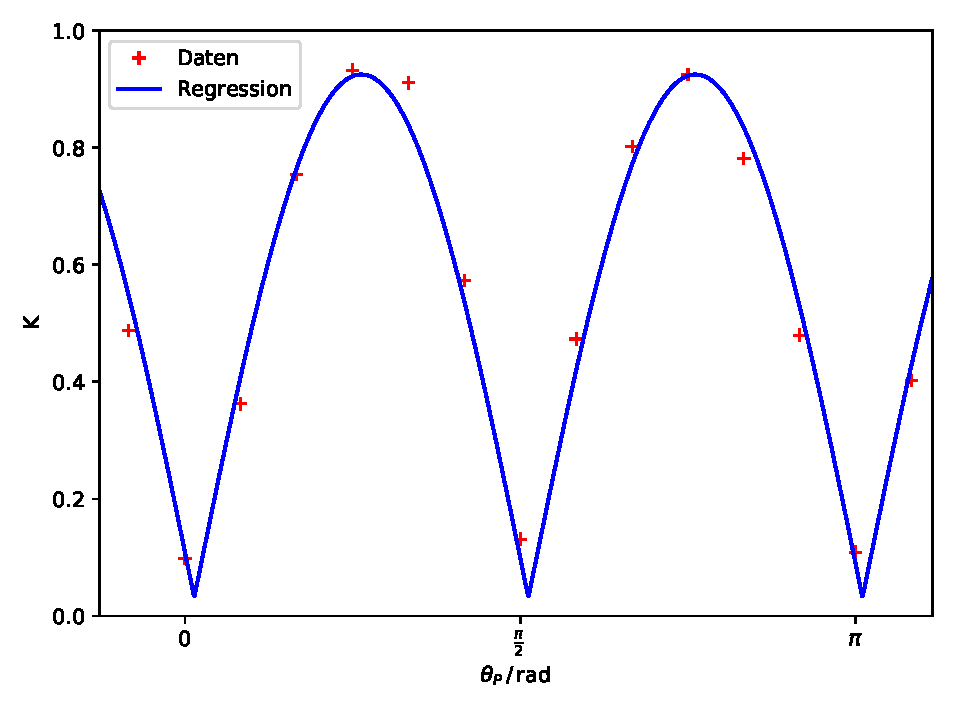
\includegraphics[width=0.7\textwidth]{Kontrast.pdf}
  \caption{Kontrast $K$ des Interferometers in Abhängigkeit von der Polarisatorstellung
  $\theta_\symup{P}$ mit Regression.}
  \label{A_abb:1}
\end{figure}

\subsection{Brechungsindex von Glas}
Um einen brauchbaren Zusammenhang zur Bestimmung des Brechungsindex der Glasplättchen
zu erhalten, sind einige Vorüberlegungen notwendig. Die Glasplättchen sind in einem
relativen Winkel $\Theta = 2 \theta_0 = 2 \cdot \SI{10}{\deg}$ zueinander
angeordnet. \eqref{T_eq:1} muss daher um
den Winkel $\pm \theta_0$ Taylorentwickelt werden. Terme ab $\theta^2$
werden dabei vernachlässigt. Es ergibt sich:
\begin{gather*}
  \mathcal{T}_{(1)}M(\theta,\theta_0) = \frac{T}{\lambda}\cdot\frac{n-1}{2n}(\theta_0^2 + 2\theta_0(\theta-\theta_0)),\\
  \mathcal{T}_{(1)}M(\theta,-\theta_0) = \frac{T}{\lambda}\cdot\frac{n-1}{2n}(\theta_0^2 - 2\theta_0(\theta+\theta_0)).
\end{gather*}
Um einen Zusammenhang für den Brechungsindex des Scheibenmaterials zu erhalten, muss
die Differenz der beiden Entwicklungen gebildet werden. Umgestellt nach $n$ folgt:
\begin{equation}
  n = \left( 1 - \frac{\lambda{M}}{2T\theta_0\theta} \right)^{-1}.
\label{A_eqn:3}
\end{equation}
Die mit \eqref{A_eqn:3} und einer Plättchendicke von $T=\SI{1}{\milli\metre}$
sowie einer Laserwellenlänge von \SI{633}{\nano\metre}
aus den Messdaten erhaltenen Werte finden sich in Tabelle
\ref{A_tab:2}, wobei $\theta_0 = \SI{138}{\deg}$ gilt und immer in \SI{2}{\deg} -Schritten
gemessen wurden. Es wurden 5 Messreihen aufgenommen. Mittelung über die Messwerte
aller Messreihen liefert einen Wert von:
\begin{equation*}
  n_\symup{Glas} = \num{1.48(3)}.
\end{equation*}

\begin{table}[h!]
  \centering
  \caption{Messwerte mit Brechungsindizes der 5 Messreihen sowie dem Mittelwert
  der Brechungsindezes $\overline{n}$ für jede Messreihe.}
  \label{A_tab:2}
  \begin{tabular}{c c || c c | c c | c c | c c | c c }
    \toprule
    & $\theta$ / \si{\deg} & $M_1$ & $n_1$ & $M_2$ & $n_2$
    & $M_3$ & $n_3$ & $M_4$ & $n_4$ & $M_5$ & $n_5$ \\
    \midrule
    & 2 & 5 & 1.35 & 7 & 1.57 & 7 & 1.57 & 6 & 1.45 & 7 & 1.57 \\
    & 2 & 6 & 1.45 & 7 & 1.57 & 6 & 1.45 & 7 & 1.57 & 6 & 1.45 \\
    & 2 & 6 & 1.45 & 5 & 1.35 & 7 & 1.57 & 5 & 1.35 & 6 & 1.45 \\
    & 2 & 7 & 1.57 & 7 & 1.57 & 7 & 1.57 & 5 & 1.35 & 6 & 1.45 \\
    & 2 & 8 & 1.71 & 5 & 1.35 & 5 & 1.35 & 7 & 1.57 & 5 & 1.35 \\
    \midrule
    $\overline{n}$ & & \multicolumn{2}{c|}{\num{1.51(7)}} & \multicolumn{2}{c|}{\num{1.48(6)}} &
    \multicolumn{2}{c|}{\num{1.50(5)}} & \multicolumn{2}{c|}{\num{1.46(5)}} &
    \multicolumn{2}{c}{\num{1.45(4)}} \\
    \bottomrule
  \end{tabular}
\end{table}

\subsection{Brechungsindex von Luft}
Messwerte und nach \eqref{T_eq:2} bestimmte Brechungsindizes sind in Tabelle
\ref{A_tab:3} dargestellt. Alle Interfernzstreifenmessungen wurden mit einem Fehler
von $\pm \, 2$ versehen, da es bei der Rückkehr auf Umgebungsdruck in der Gaszelle
zu Fehlzählungen kommt. Die Länge der Zelle beläuft sich auf $L = \SI{10}{\centi\metre}$.
Wieder beträgt die Laserwellenlänge \SI{633}{\nano\metre}.\\
Es ergibt sich also ein Wert von
\begin{equation*}
  n_\symup{Luft} = \num{1.000264(7)}.
\end{equation*}

\begin{table}[h!]
  \centering
  \caption{Gezählte Interferenzstreifen $M$ mit berechneten
  Brechungsindizes für Luft und Mittelwert $\overline{n}$.}
  \label{A_tab:3}
  \begin{tabular}{c c c}
    \toprule
    & $M$ & $n$ \\
    \midrule
    & 42 $\pm$ 2 & \num{1.000266(13)} \\
    & 41 $\pm$ 2 & \num{1.000260(13)} \\
    & 42 $\pm$ 2 & \num{1.000266(13)} \\
    \midrule
    $\overline{n}$ & & \num{1.000264(13)}\\
    \bottomrule
  \end{tabular}
\end{table}

\section{Diskusion}
\begin{table}[h!]
  \centering
  \caption{Übersicht über die Messergebnisse mit Literaturwerten.}
  \label{D_tab:1}
  \begin{tabular}{c c c}
    \toprule
    & Messung & Literatur \\
    \midrule
    $n_\symup{Glas}$ & \num{1.48(3)} & \num{1.5} \cite[S. 11-5]{anleitung}  \\
    $n_\symup{Luft, \SI{633}{\nano\metre}}$ & \num{1.000264(13)} & \num{1.000277} \cite{Luft} \\
    \bottomrule
  \end{tabular}
\end{table}

Mess- und Literaturwerte finden sich in Tabelle \ref{D_tab:1}. Es zeigt sich, dass
die Literaturwerte für beide Messungen in der Messungenauigkeit liegen. Da die Glassorte
nicht bekannt ist, kann der angegebene Literaturwert für die Glasmessung nur als
Richtwert genommen werden. Jedoch liegen auch Literaturwerte für häufig anzutreffende
Glasarten bei einer Wellenlänge von \SI{633}{\nano\metre} im Bereich der Messungenauigkeit
(beispielsweise $n=\num{1.52}$ ($\num{1.4}\sigma$) für Kalk-Natron-Glas / Normalglas \cite{KNG} oder
$n=\num{1.46}$ für Quarzglas \cite{QG})\\
Bei der Messung des Brechnungsindex von Luft konnte das Fehlerintervall nur getroffen
werden, da die Interfernzstreifenzählung nicht als Fehlerfrei angesehen werden konnte
und ein pauschaler Fehler von $\pm \, 2$ angeommen wurde.
Bei Wiederbefüllen der Gaszelle stieg wärend
den letzten ca. \SI{100}{\milli\bar} vor Umgebungsdruck die Füllrate der Zelle rasant an.
Es konnte jedoch beobachet werden, dass die dadurch entstehenden Interfernzstreifen
von der Ausleseelektronik nicht aufgenommen werden konnten. Hier ist daher mit
systematischen Fehlern zu rechnen. Für aussagekräftigere Werte wäre eine erneute
Messung notwendig.\\


\newpage
\nocite{*}
\printbibliography
